\documentclass[aspectratio=169]{beamer}

\usetheme{default}
\setbeamertemplate{navigation symbols}{}
\setbeamertemplate{enumerate item}{\color{navy}\arabic{enumi}.}
\setbeamertemplate{itemize item}{\color{black}\textbullet}
\setbeamertemplate{itemize subitem}{\color{black}\textbullet}
\usepackage{booktabs}
\usepackage{xcolor}
\usepackage{graphicx}
\definecolor{navy}{RGB}{0, 0, 128}
\definecolor{lightblue}{RGB}{230,240,250}

\usepackage{hyperref}
\hypersetup{
    colorlinks=true,
    linkcolor=navy,
    urlcolor=navy,
    citecolor=navy
}

\begin{document}

\begin{frame}

\begin{itemize}
\itemsep1.5em
\item<1-> Major advantage of elicited probabilities: handling unobserved heterogeneity
\item<2-> We can say more because we have more information about preferences
\item<3-> Stated probabilities contain more information than 0/1 or rank ordering
\item<4-> Can estimate nonparametric mixing distributions:
\item<5-> Simply estimate individual-specific $\gamma$'s
\item<6-> Resulting distribution is almost never normal (i.e. it's skewed, leptokurtic, etc.)
\end{itemize}

\end{frame}

\begin{frame}

Example from \href{https://www.sciencedirect.com/science/article/abs/pii/S0304407621000415}{Ko\c{s}ar et al. (2022)}

\bigskip

\begin{columns}[T]
\begin{column}{0.6\textwidth}
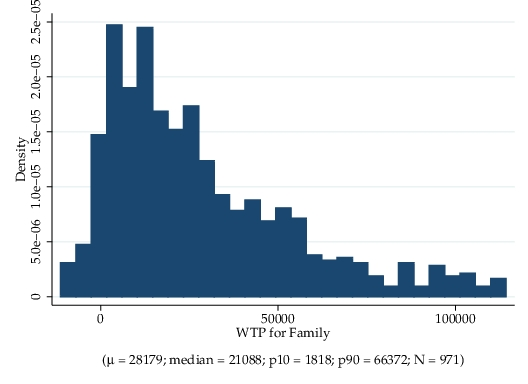
\includegraphics[width=\textwidth]{histo_wtp_family.jpg}
\end{column}
\begin{column}{0.4\textwidth}
\begin{itemize}
\itemsep1.5em
\item<2-> The WTP distribution is highly skewed
\item<3-> Some people \textit{really} like living close to family
\item<4-> Some people prefer to be apart from family\par (negative WTP)
\end{itemize}
\end{column}
\end{columns}

\end{frame}

\begin{frame}
\begin{itemize}
\itemsep1.5em
\item<1-> Stated probabilistic choice experiments are not a silver bullet
\item<2-> You're still reduced to the SP vs. RP conundrum
\item<3-> Will people actually do what they told you they would do?
\item<4-> To resolve this, most studies have to conduct follow-on surveys
\item<5-> Rationale: in between survey waves, people make actual choices
\item<6-> You can then see how well their SP compares to their RP
\item<7-> I've never seen SP diverge from RP, but that could be due to publication bias
\end{itemize}

\end{frame}


\begin{frame}

Other details for estimation

\bigskip

\begin{itemize}
\itemsep1.5em
\item<2-> You need to bootstrap to get appropriate standard errors
\item<3-> This is because you have panel data
\item<4-> Cluster (at individual level) robust inference won't be enough
\item<5-> To get individual-specific preference estimates, \texttt{qreg} at individual level
\end{itemize}

\end{frame}

\begin{frame}

Papers that use stated probability experiments

\bigskip

\begin{itemize}
\itemsep1.5em
\item<2-> \href{https://onlinelibrary.wiley.com/doi/full/10.1111/j.1468-2354.2010.00586.x}{Blass, Lach \& Manski (2010, IER)}: valuing electricity reliability
\item<3-> \href{https://www.sciencedirect.com/science/article/abs/pii/S0261379415000086}{Delavande \& Manski (2015, JPE)}: election participation
\item<4-> \href{https://academic.oup.com/qje/article/133/1/457/4095201}{Wiswall \& Zafar (2018, QJE)}: job choice
\item<5-> \href{https://www.journals.uchicago.edu/doi/full/10.1086/701808}{Delavande \& Zafar (2019, JPE)}: university choice
\item<6-> \href{https://www.sciencedirect.com/science/article/abs/pii/S0304407621000415}{Ko\c{s}ar et al. (2022, Journal of Econometrics)}: migration within US
\item<7-> Many others
\end{itemize}

\end{frame}

\end{document}